% !TEX root = main.tex
\chapter{Theory}

	Understanding the theory behind the rocket's flow requires a basic knowledge of rockets. Therefore, the first theoretical segment concerns basic rocketry, followed by a more advanced segment of nozzle theory.

\section{Basic Rocket Science}

	A rocket engine consists of a few fundamental elements. There exists two types of rocket engines, as seen in figure \ref{fig:rocketvsduct}. A rocket engine is a type of jet engine that, in contrast to duct jets, carry their own rocket propellant. Jet engines as seen in aeroplanes are usually situated with a duct, confining the air flow. Rocket engines on the other hand carry a supply of oxygen and rocket propellant, which allows them to function even in vacuum.

	\begin{figure}
		\centering
		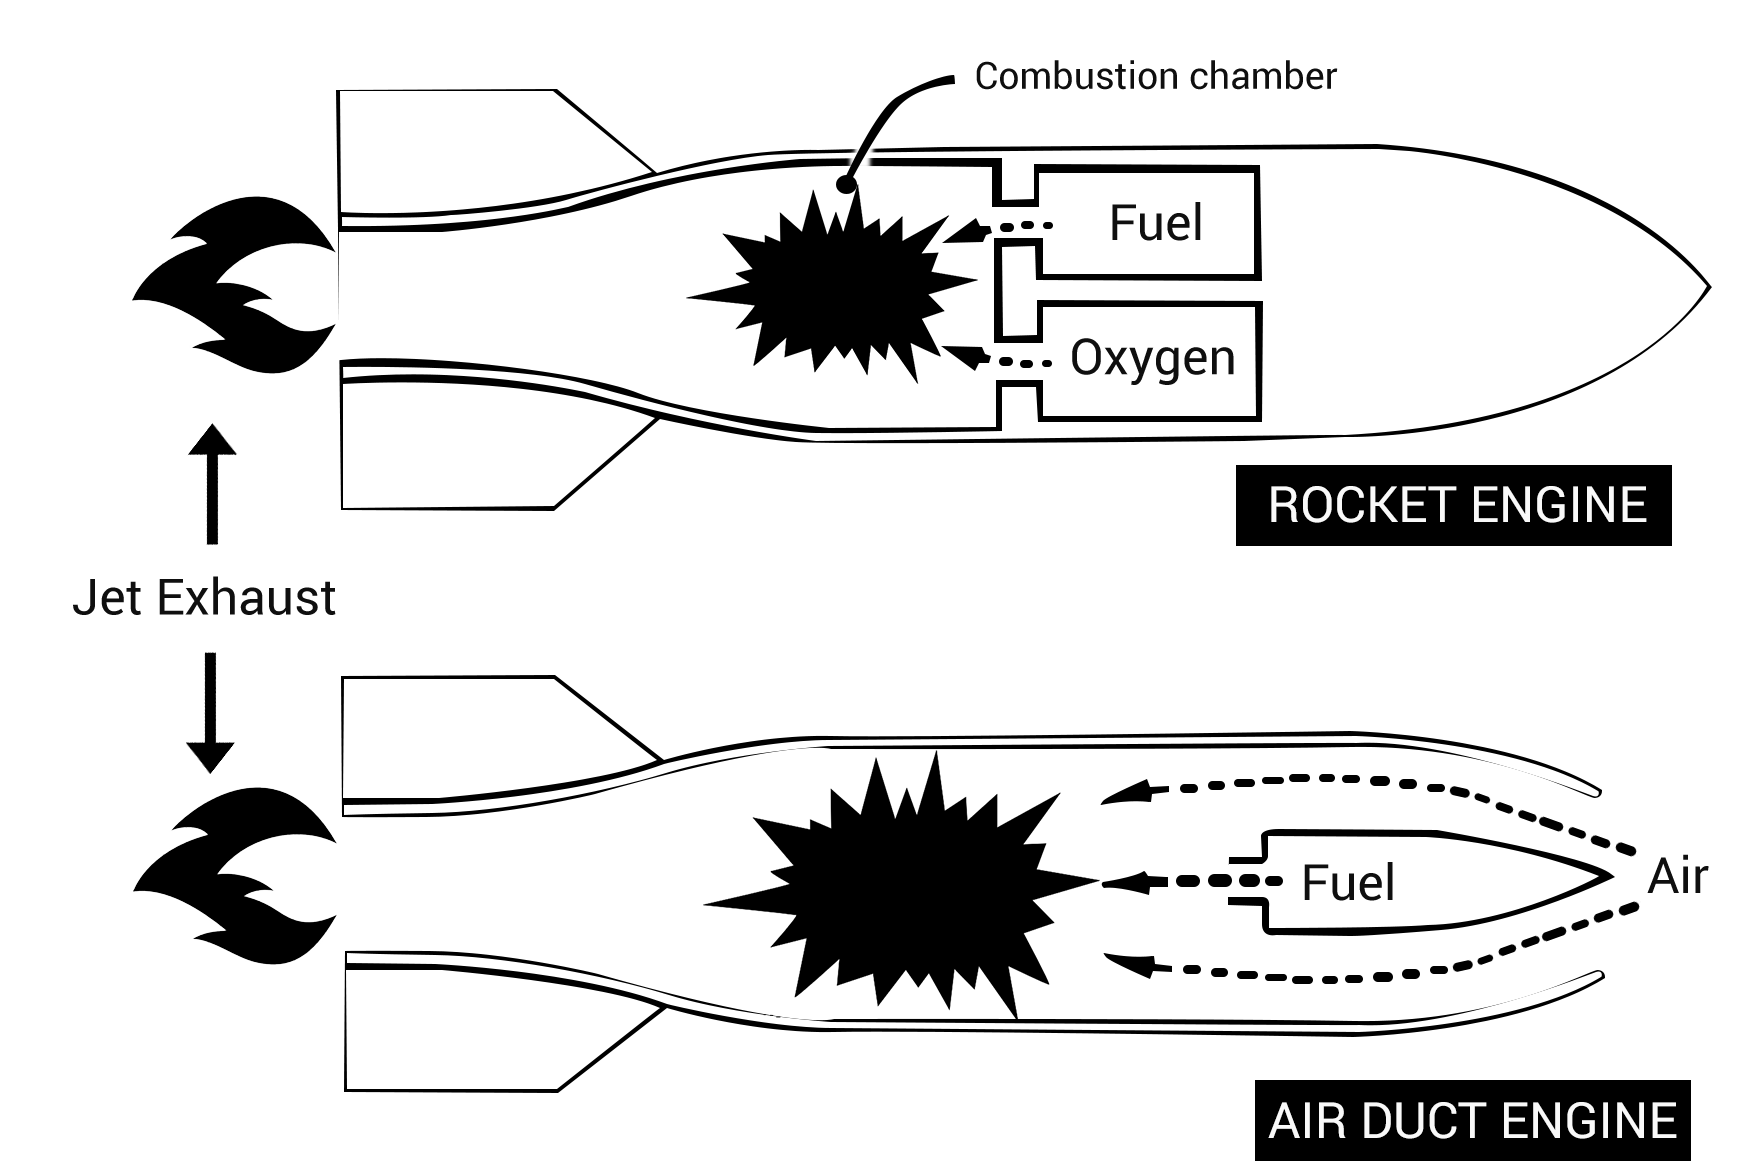
\includegraphics[width=\textwidth]{rocketvsduct}
		\caption{Schematic difference of the two types of jet engines: Rocket engines and air duct engines.}
		\label{fig:rocketvsduct}
	\end{figure}

	Rocket engines work by obtaining thrust in accordance with Newton's third law. The internal combustion chamber accelerates fluids through a propelling nozzle to high speeds. The fluid is most often a gas created from mixing fuel and oxidizing components in a the combustion chamber. The exhaust is accelerated to supersonic speeds by expansion in the nozzle, which forces the engine in the opposite direction.

	Most rockets used today are liquid rockets which store their propellant and oxidizing component in separate tanks. The liquid fuel is then forced into the combustion chamber for consumption. Solid-fuel rockets contain propellant prepared with a fixed fuel and oxidizing component. The fuel is called 'grain', and the storage compartment for the grain is the combustion chamber. A hybrid rocket is the mixture between the two. Most often, hybrid rockets contain a solid fuel, or 'grain' and liquid or gaseous oxygen, thus earning the name hybrid engine. Variations of this engine type do exist, but this configuration is the most often used \cite{rockProp}. Solid oxidizers are uncommon as they are problematic and have worse performance than liquid oxidizers.

	Liquid and hybrid engines both use injectors to disperse oxygen and propellant into the combustion chamber. For a hybrid engines, this means spreading oxygen to the grains surface to allow combustion.

	Hybrid rockets are inherently safer than its two counterparts, and accidents are less volatile as accidental fuel mixing is a non-issue.\footnote{Assuming you can control the oxidizer inlet valve.} The oxidizer and fuel are almost always contained in separate chambers, which also reduces the mechanical complexity of the rocket in comparison to liquid rockets.

\section{Hybrid Rocket Engine}

\begin{figure}
	\centering
	\includegraphics[width=\textwidth]{rocketsideview}
	\caption{The hybrid rocket built at Navitas in Aarhus for educational purposes.}
	\label{fig:rocketpic}
\end{figure}

	The hybrid rocket engine consists of three parts: The combustion chamber, the converging into a throat, and diverging section after called the nozzle. A rocket's effectivity is highly dependent on the shape, size and ratios between these three segments. Accordingly, it is imperative to study these parts of the rocket's design.

	The rocket in question is seen in figure \ref{fig:rocketpic} which is divided into a tank, three chambers and a nozzle. A schematic setup can be seen in figure \ref{fig:crosssect}.

	\begin{figure}
		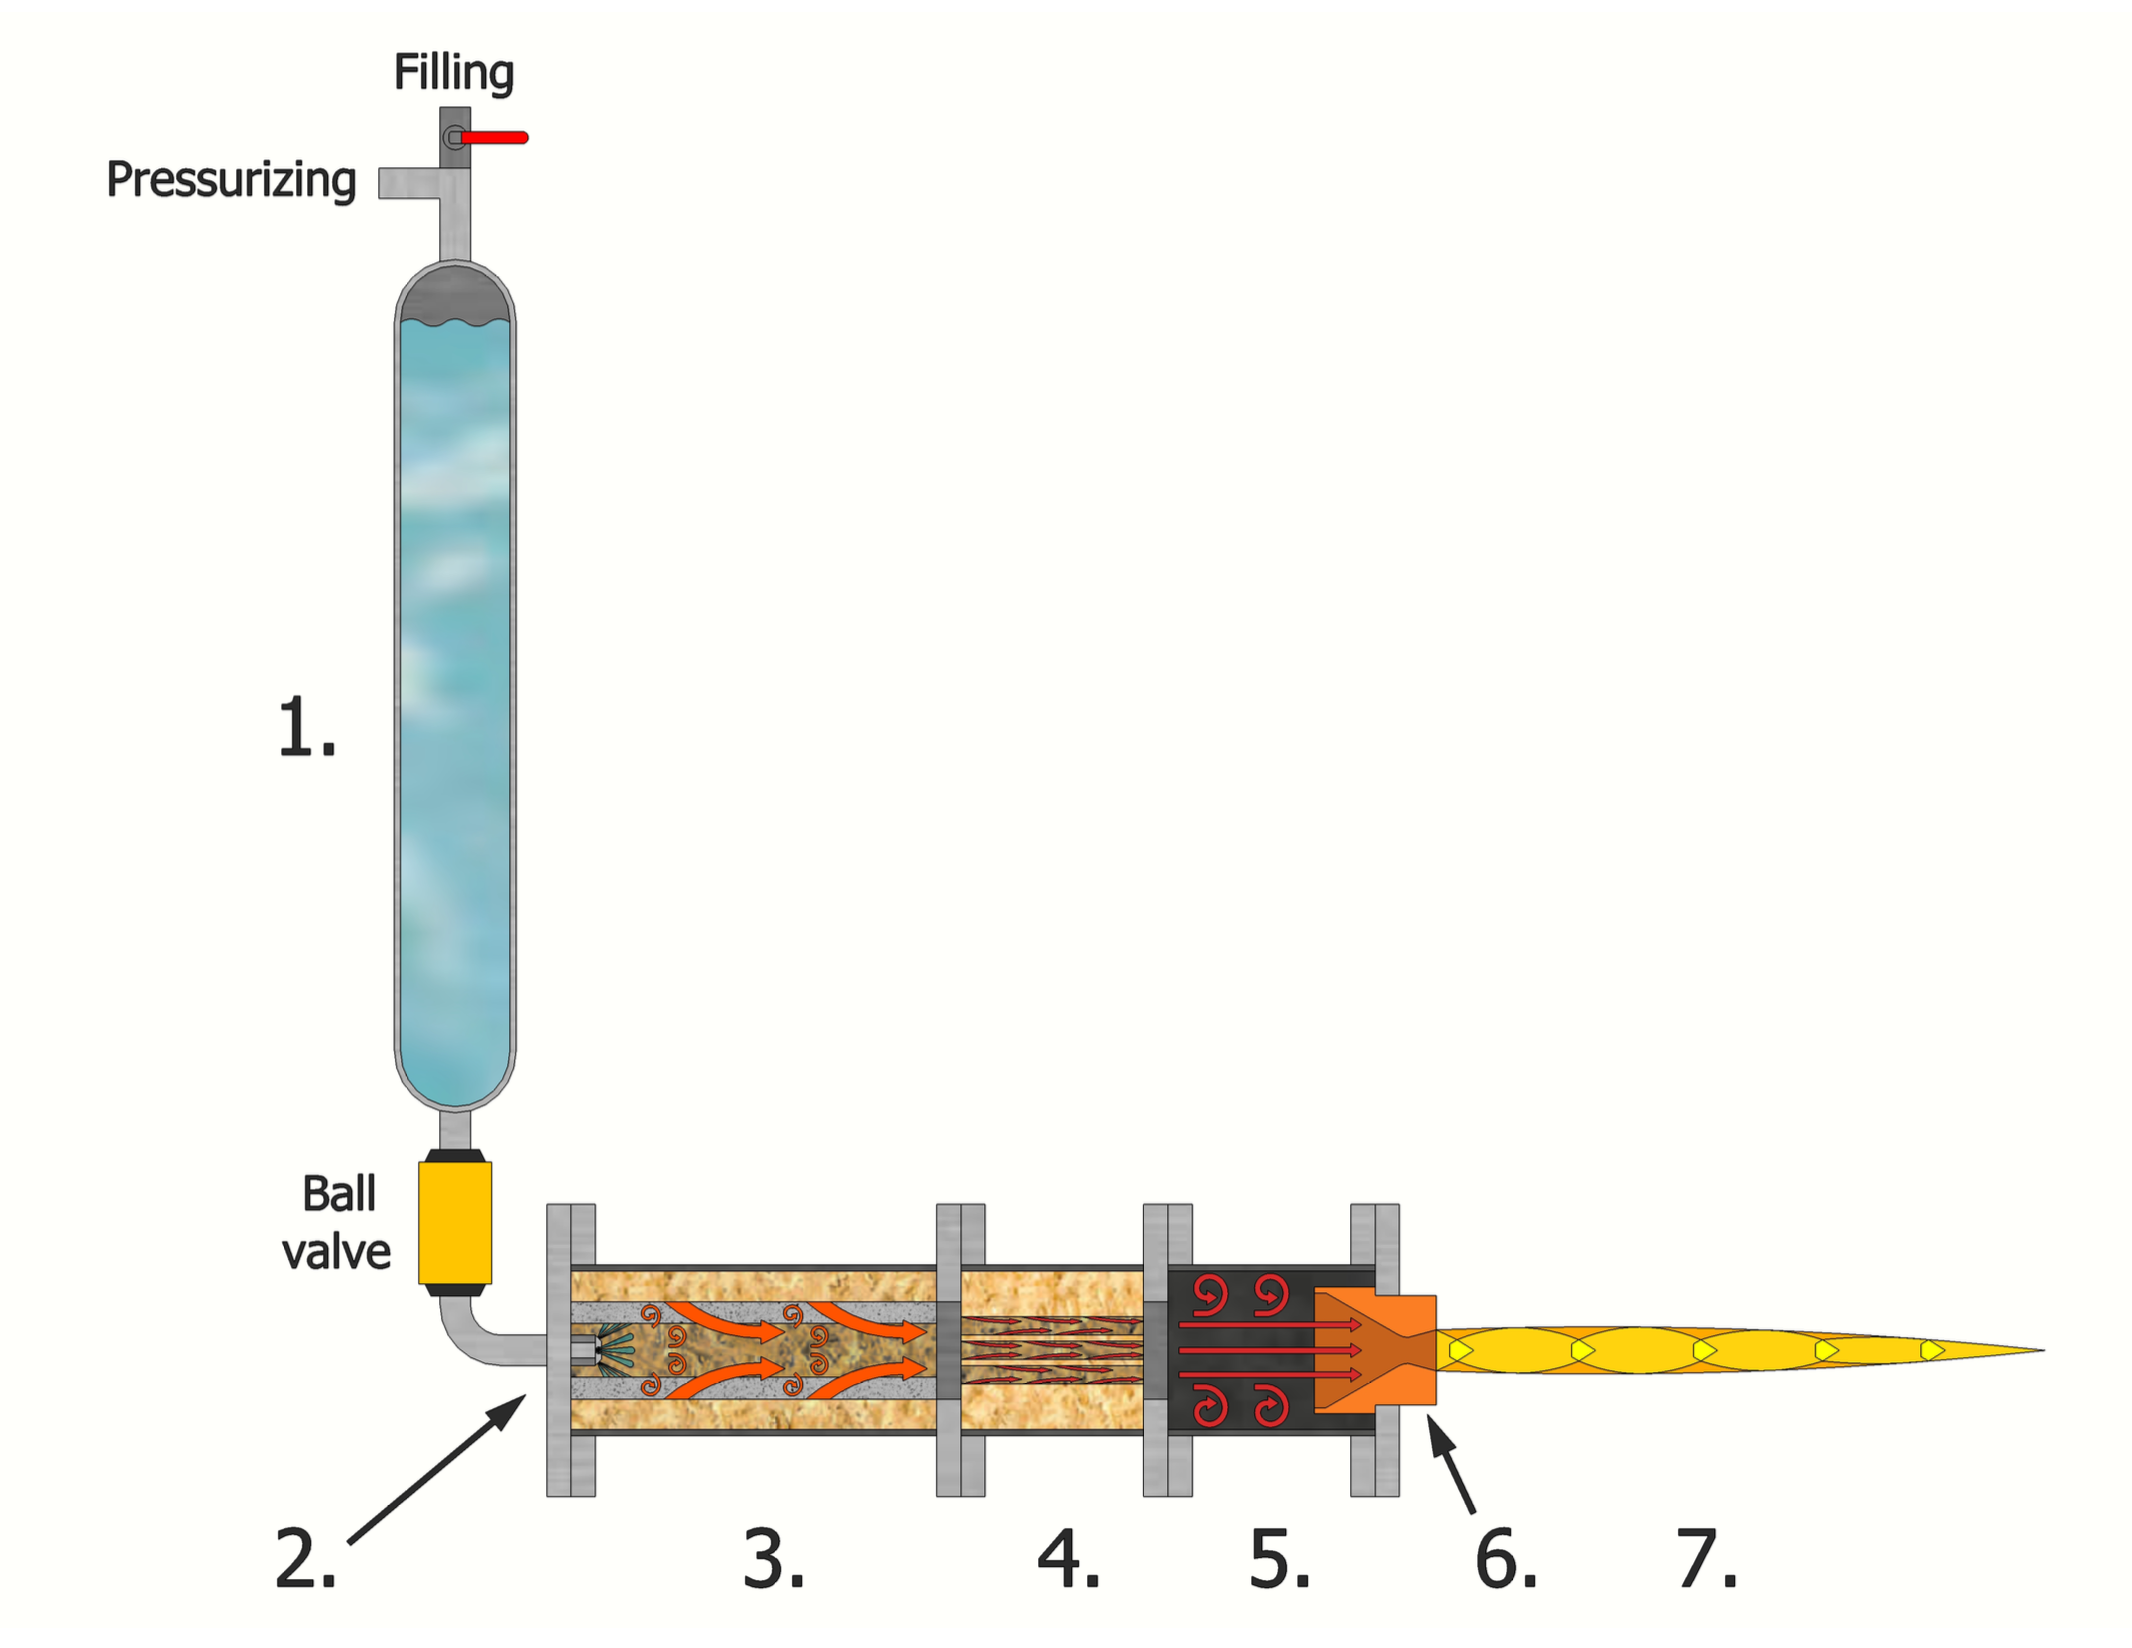
\includegraphics[width=\textwidth]{crosssect}
		\caption{Cross section of the rocket.}
		\label{fig:crosssect}
	\end{figure}

	From the left: The tall tank marked with a $1.$ contains the oxidizing agent, which is injected into the first part of the rocket. The oxidizing agent used is hydrogen peroxide in an $80\%$ concentration. Point $2.$ marks the place where the injecting nozzle is placed, which determines the rocket's mass flow rate. The longest part of the rocket, as seen on figure \ref{fig:crosssect} marked with $3.$, contains potassium permanganate engulfed in a flame retardant foam. The mixing of potassium permanganate and hydrogen peroxide rapidly creates large amounts of oxygen, which is forced through the rocket's second part: the grain chamber, marked with numer $4.$ The rocket's main fuel is plain Medium-Density Fiberboard (MDF), which resides here. The energy released during decomposition heats the wooden MDF grain, until temperatures reach MDF's autoignition point of 492K at atmospheric oxygen levels \cite{mdfAIT}. Around this point the fuel combusts, and the exhaust exits through the nozzle $6.$ after it has passed the mixing chamber $5$.

	All calculations and considerations made in the report is in regard to this particular rocket. The following subsections each elaborate individual segment of the rocket, with the purpose of providing the necessary background knowledge to understand the ignition simulations and results. The explanation is given step by step, starting with injection and ending with exhaustion.


\subsection{Injection}

	To initiate combustion in the hybrid engine, an oxidizer is injected into the combustion chamber. The rocket in question creates its oxydizer by mixing an oxidizing agent with potassium permanganate. The agent is contained in a pressurized tank containing an $80 \%$ \chem{H_2O_2} rich mixture with the remainder being \chem{H_2O}. The oxidizing agent is assumed to be injected at a constant rate of:
		\begin{align}
			\dot{m}_\text{injection} = \SI{0.246}{\kg\per\s}.
		\end{align}
	in accordance to data collected at the recent launch \cite{Alex2015rapport}.

	The oxidizing agent is injected into the first chamber where decomposition into \chem{O_2} is aided by potassium permanganate. The hydrogen-peroxide (\chem{H_2O_2}) decomposes into dioxygen (\chem{O_2}) as it reacts with the potassium permanganate (\chem{K Mn O_4}), which is encased in a flame retardant foam. The balanced chemical redox reaction is as follows:
		\begin{align}
			\chem{6 KMnO_4 + H_2O_2} &\rightarrow \chem{3 K_2O_2 + 6 MnO_2 + H_2O + 3 O_2}
		\end{align}
	The specific enthalpy released during decomposition is:
		\begin{align}
			\Delta h_\text{decomposition} &= \frac{\Delta H_\chem{H_2O_2}}{\text{M}_\chem{H_2O_2}}
		\end{align}
	Where $\Delta H$ is the change in enthalpy. The energy released heats the grain's surface to autoignition temperatures of approximately $\SI{220}{\celsius}$ in this extremely oxygen-rich environment. The increased temperature increases the pressure, in accordance to the ideal-gas law:
		\begin{align}
			P V &= n R T
		\end{align}
	Which is assumed to be valid as the gas is approximately stagnant in the mixing chamber \cite{atkins}.
	The ideal gas law is crucial in our description of the rocket. Describing the rocket's upstart phase requires coupling the changes in temperature $T$, pressure $P$ and amount of substance $n$. During injection and decomposition, combustion occurs simultaneously.

	\subsection{Combustion Chamber}

		The combustion chamber contains two important theoretical aspects. First, the propellant grain has significant effects on the rocket's thrust over time. Secondly, the theoretical description of the rocket's combustion allows us to estimate different working parameters, and deciding the rocket nozzle's size and area ratios.

	\subsubsection{Propellant Grain}

		The combustion chamber consists of an approximate 3 liter cavity which is filled with the grain. The actual volume in a hybrid rocket depends strongly on the initial condition of the grain and the fuel's combustion rate. Holes have to be carved in the grain to allow oxygen to reach the grain's surface, and transport exhaust towards the throat. The combustion rate is largely determined by the exposed surface area of the grain, and the flux of the oxidizer. The surface gradually expands as the outer regions are burned away, thus changing the rocket's effective thrust over time \cite{ignition}. The propellant's increase in burning area during ignition is assumed to be negligible, compared to the rapid increases in pressure and temperature.

				\begin{figure}
					\centering
					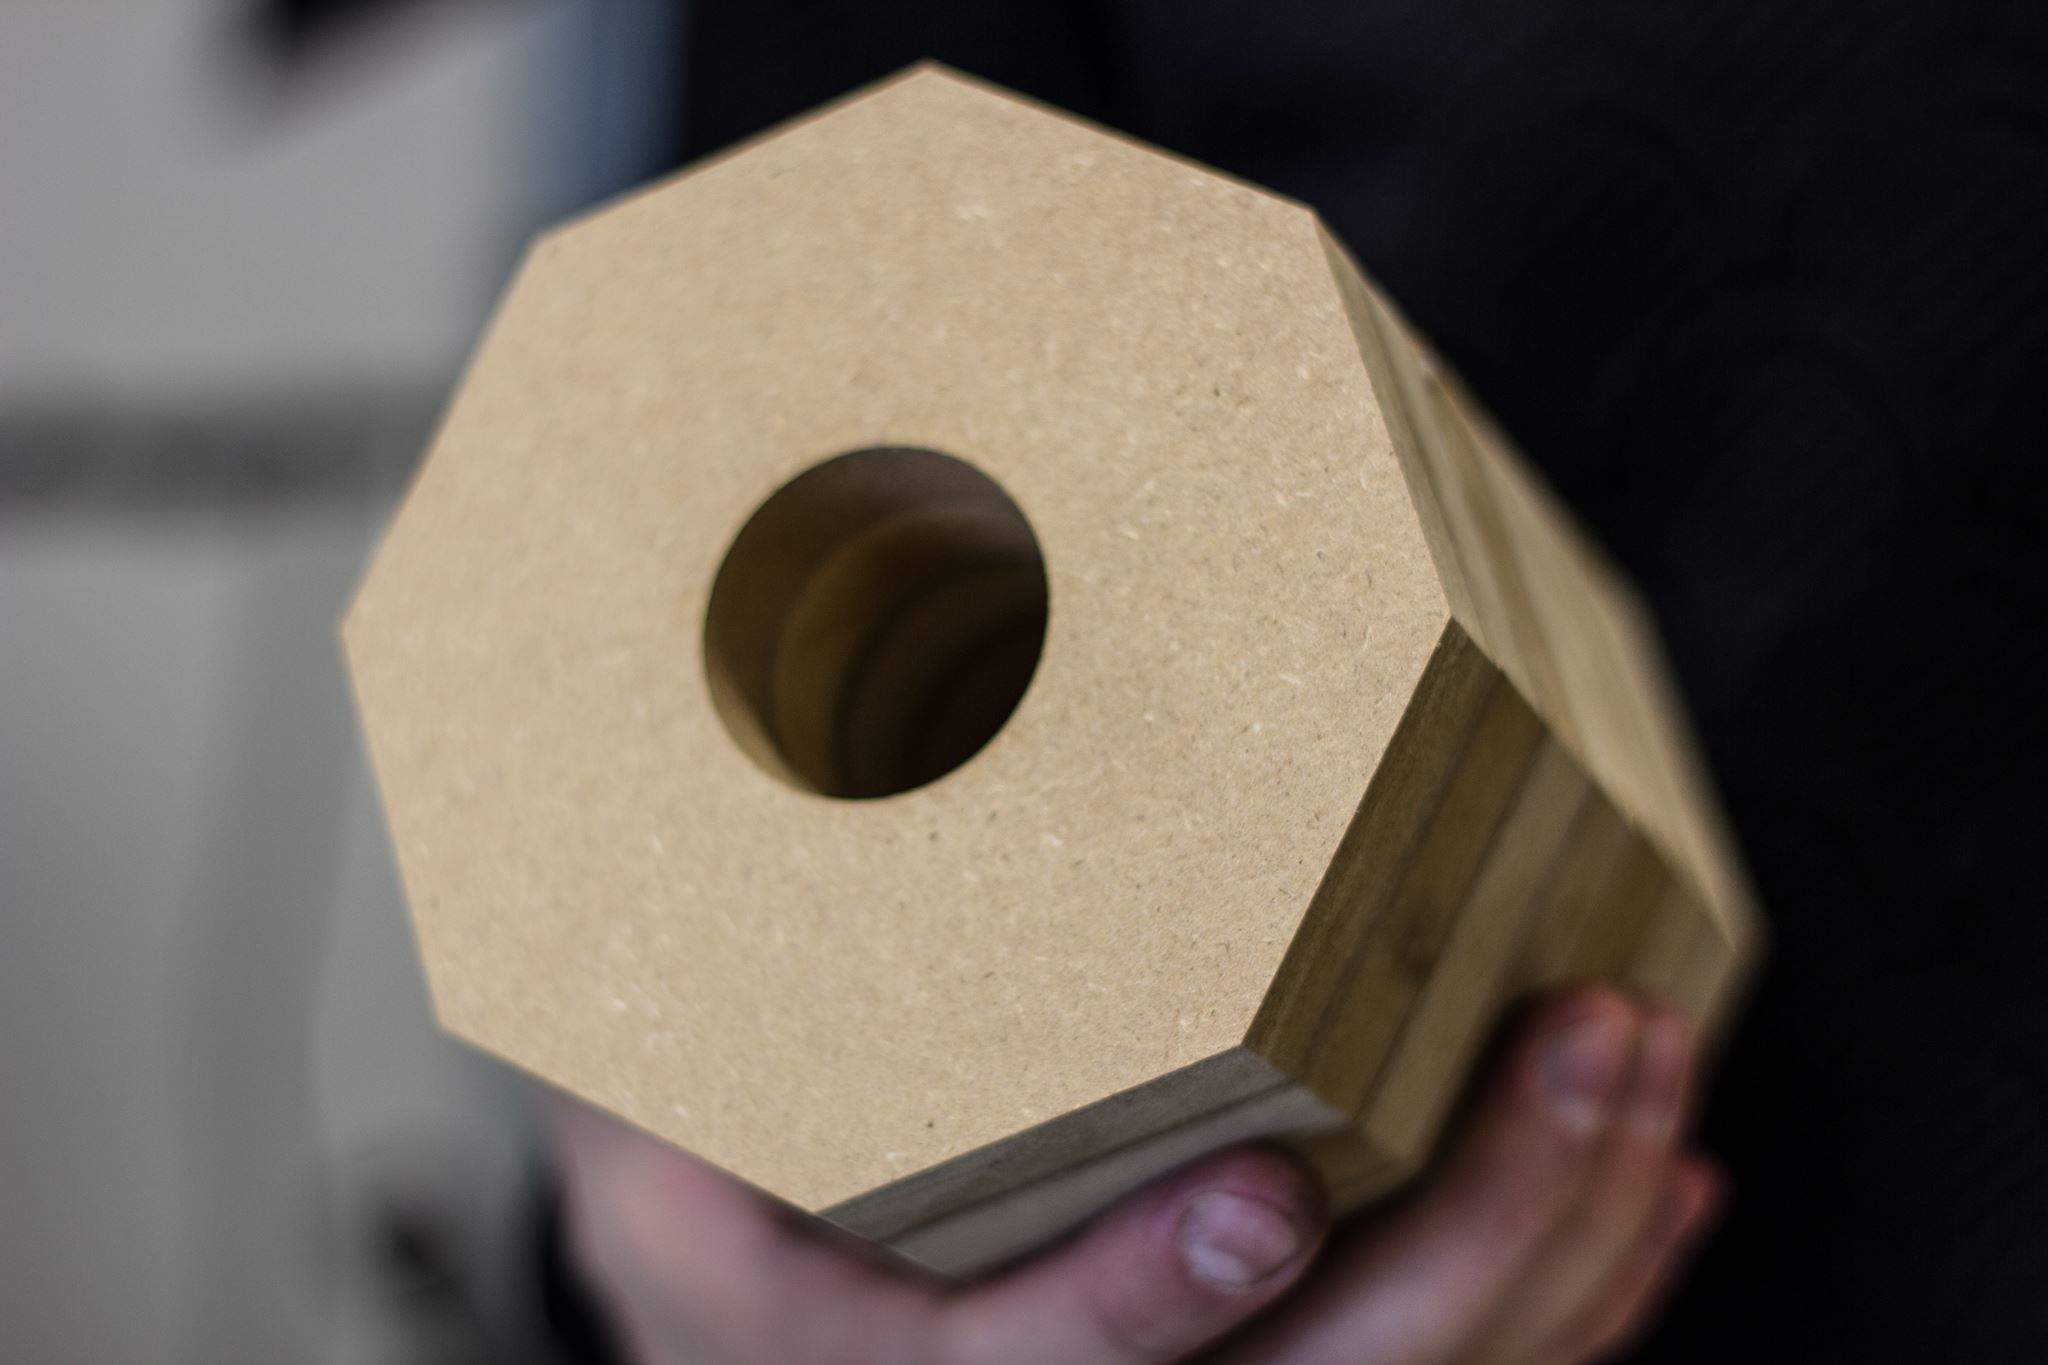
\includegraphics[width=\textwidth]{singlehole}
					\caption{Example of MDF grain with a single combustion--hole. This will have a uniformly increasing regression-rate, as the burning area increases evenly.}
					\label{fig:singlehole}
				\end{figure}

		The shapes and sizes of the holes in the grain has a large impact on the initial ignition and thrust ratios \cite{nakka}. An example of a single hole configuration can be seen in figure \ref{fig:singlehole}, and more examples can be found on \url{http://www.nakka-rocketry.net/th_grain.html}, along with a general performance description. Depending on the surface areas and designs, the different grain's regression rate varies greatly over time. The regression rate will be proportional to the thrust, unless oxygen is the limiting factor. The generated thrust is directly proportional to the instantaneous burning area, and as this area increases, so does the thrust.

			\begin{figure}
				\centering
				
\includegraphics[width=\textwidth]{wagonwheel}
				\caption{The wagon-wheel design used in all rocket tests concluded in this report. The large surface area allows combustion on a larger surface, which gives more effective combustion.}
				\label{fig:wagonwheel}
			\end{figure}

		An alternative explanation to the pressure spike could therefore be a very fast increase in regression area. The grain's specifications from the previous tests are not mentioned, but a wagon--wheel design as seen in figure \ref{fig:wagonwheel} with several holes could allow ignition in single canals before all of them. This could allow hot pyrolytic fuel and oxygen to accumulate, causing an eventual explosion. The large surface area of the wagon--wheel design is allows for cleaner, more efficient combustion, and it is therefore the preferred setup for our experiments \cite{nakka}.

	\subsubsection{Autoignition}

		There are two types of ignition: Autoignition and piloted ignition \cite{principlesoffire}. Piloted ignition is the process of flame propagation in a premixed fuel system, such as lighting a candle or starting a petrol engine. This is the usual way of igniting every day systems, however, MEOWTH uses the other type: Autoignition.

		Autoignition occurs without a spark of flame present. The fuel must have a certain concentration and temperature, before spontaneously igniting. This temperature is lowered by rising oxygen concentration and pressure, which complicates setting a specific point of time of ignition \cite{ASTMautoign}. According the the MDF's datasheet \cite{mdfAIT}, autoignition occurs around \SIrange{220}{250}{\celsius}. This minimum temperature tells us when spontaneous combustion takes place, the question is then how quickly after reaching this temperature does the material ignite?

		Autoignition time $t_\text{auto}$ for thick materials (thicker than $\SI{2}{mm}$) is given by:
		\begin{align*}
			t_\text{auto} &= C (k \rho c) \left[\frac{T_\text{auto} - T_\text{initial}}{\phi} \right]^2
		\end{align*}
		where $k$ is the thermal conductivity of the material, $C$ is a constant depending on the heat flux, but roughly equivalent to $0.785$ assuming no heat loss \cite{principlesoffire}. $T_\text{auto}$ is the autoignition temperature and $T_\text{initial}$ is the starting temperature, and $\phi$ is the heat flux.

		Back--of--the--envelope calculations shows that the autoignition time is on the order of magnitude $\SI{10^{-5}}{\s}$, which is way faster than anything we should be able to measure. The temperature and pressure rise far too quickly for this to have an obvious effect on the ignition. It is thus assumed to be far too small to have any real influence, compared to the autoignition temperature.

	\subsubsection{Combustion}

		As temperatures reach the MDF's autoignition point, and oxygen levels increase, combustion starts taking place. The combustion reaction can be described chemically by the formula:
			\begin{align}
				\chem{C_3 H_4 O_2 + 3 O_2} &\rightarrow \chem{3 CO_2 + 2H_2O}
			\end{align}
		Energy released in this reaction heats up the chamber's fluids towards a design temperature of $\SI{2498}{K}$. Assuming a \emph{closed} chamber, the rise in temperature and amount of substance yields a rapid increase in pressure over time. This is not a desired property, as that would eventually lead to engine destruction. The accumulated decomposed and combusted material leaves through the rocket's throat, which allows the rocket to reach pressure-equilibrium. The throat's area is essential to the rocket's pressure and thus stability, hence the advance to the throat.

\subsection{Throat}

	The throat begins at the end of the combustion chamber, at the opposite side of where injection occurs. The throat is characterized by the convergence of the rocket chamber into a small passage called the throat, followed by a diverging section: The nozzle. The throat can be seen schematically on figure \ref{fig:delaval}. The throat's cross-sectional area is what determines the maximum flow rate, as the speed of sound restricts the flow of matter. In order to calculate the amount of matter contained in the chamber, it is crucial to know how much is flowing out. Due to conservation of mass, the flow rate $\dot{m}_t$ must be proportional to the density of the material, the velocity and the throat's area according to \cite{nasacompflow}:
		\begin{align}
			\dot{m}_t &= \rho_t \cdot v_t \cdot A_t
		\end{align}
		The velocity $v_t$ is thus roughly proportional to the mass flow as the area and density are approximately constant in this case. Hence, as the matter approaches the speed of sound, the flow rate out of the rocket stagnates. This is called mass flow choking, which must be at a maximum when the velocity is equal to the speed of sound. This condition is satisfied when the mach number $M=1$. For an ideal compressible gas, this becomes:
		\begin{align}
			\dot{m}_t &= \frac{A_t P_c}{\sqrt{T_t}} \sqrt{\frac{\gamma}{\text{R}}} \left(\frac{\gamma+1}{2}\right)^{-\frac{\gamma+1}{2(\gamma-1})}
		\end{align}
	Where $P_c$ is the pressure in the combustion chamber, $T_t$ is the temperature in the throat, $\gamma$ is the specific heat ratio and R is the gas constant \cite{nasacompflow}. Three outcomes are possible:
	\begin{align*}
		\dot{m}_t < \dot{m}_{in} & ~,~ \text{less mass is coming out than is flowing "into" the rocket.} \\
		\dot{m}_t = \dot{m}_{in} & ~,~ \text{mass outflow equilibrium.} \\
		\dot{m}_t > \dot{m}_{in} & ~,~ \text{more mass is flowing out than is being created.}
	\end{align*}
	The first outcome would yield increasing pressure until the rocket has burned all of it's fuel, or it explodes. The second option is what we know as a safe and steady rocket, assuming the designed mass flow equilibrium is within the rocket's boundaries. The final outcome will yield a slow decrease in pressure over time, until the rocket has been exhausted for material inside and combustion ceases. \fxnote{Passer det med masse?}

	In order to describe the initial pressure spike it is necessary to not assume any of these conditions. The abrupt change from the first to the second condition was initially hypothesized to cause the spike in pressure. Therefore, simulating the mass flow out of the rocket is essential to our understanding of the phenomenon. This does however require knowledge of several key parameters within the rocket, which are difficult to calculate, unless some things are assumed, such as conservation of entropy. However, in order to combine this knowledge, we first have to look at the final piece of theory.

\subsection{Nozzle}

	\begin{figure}
		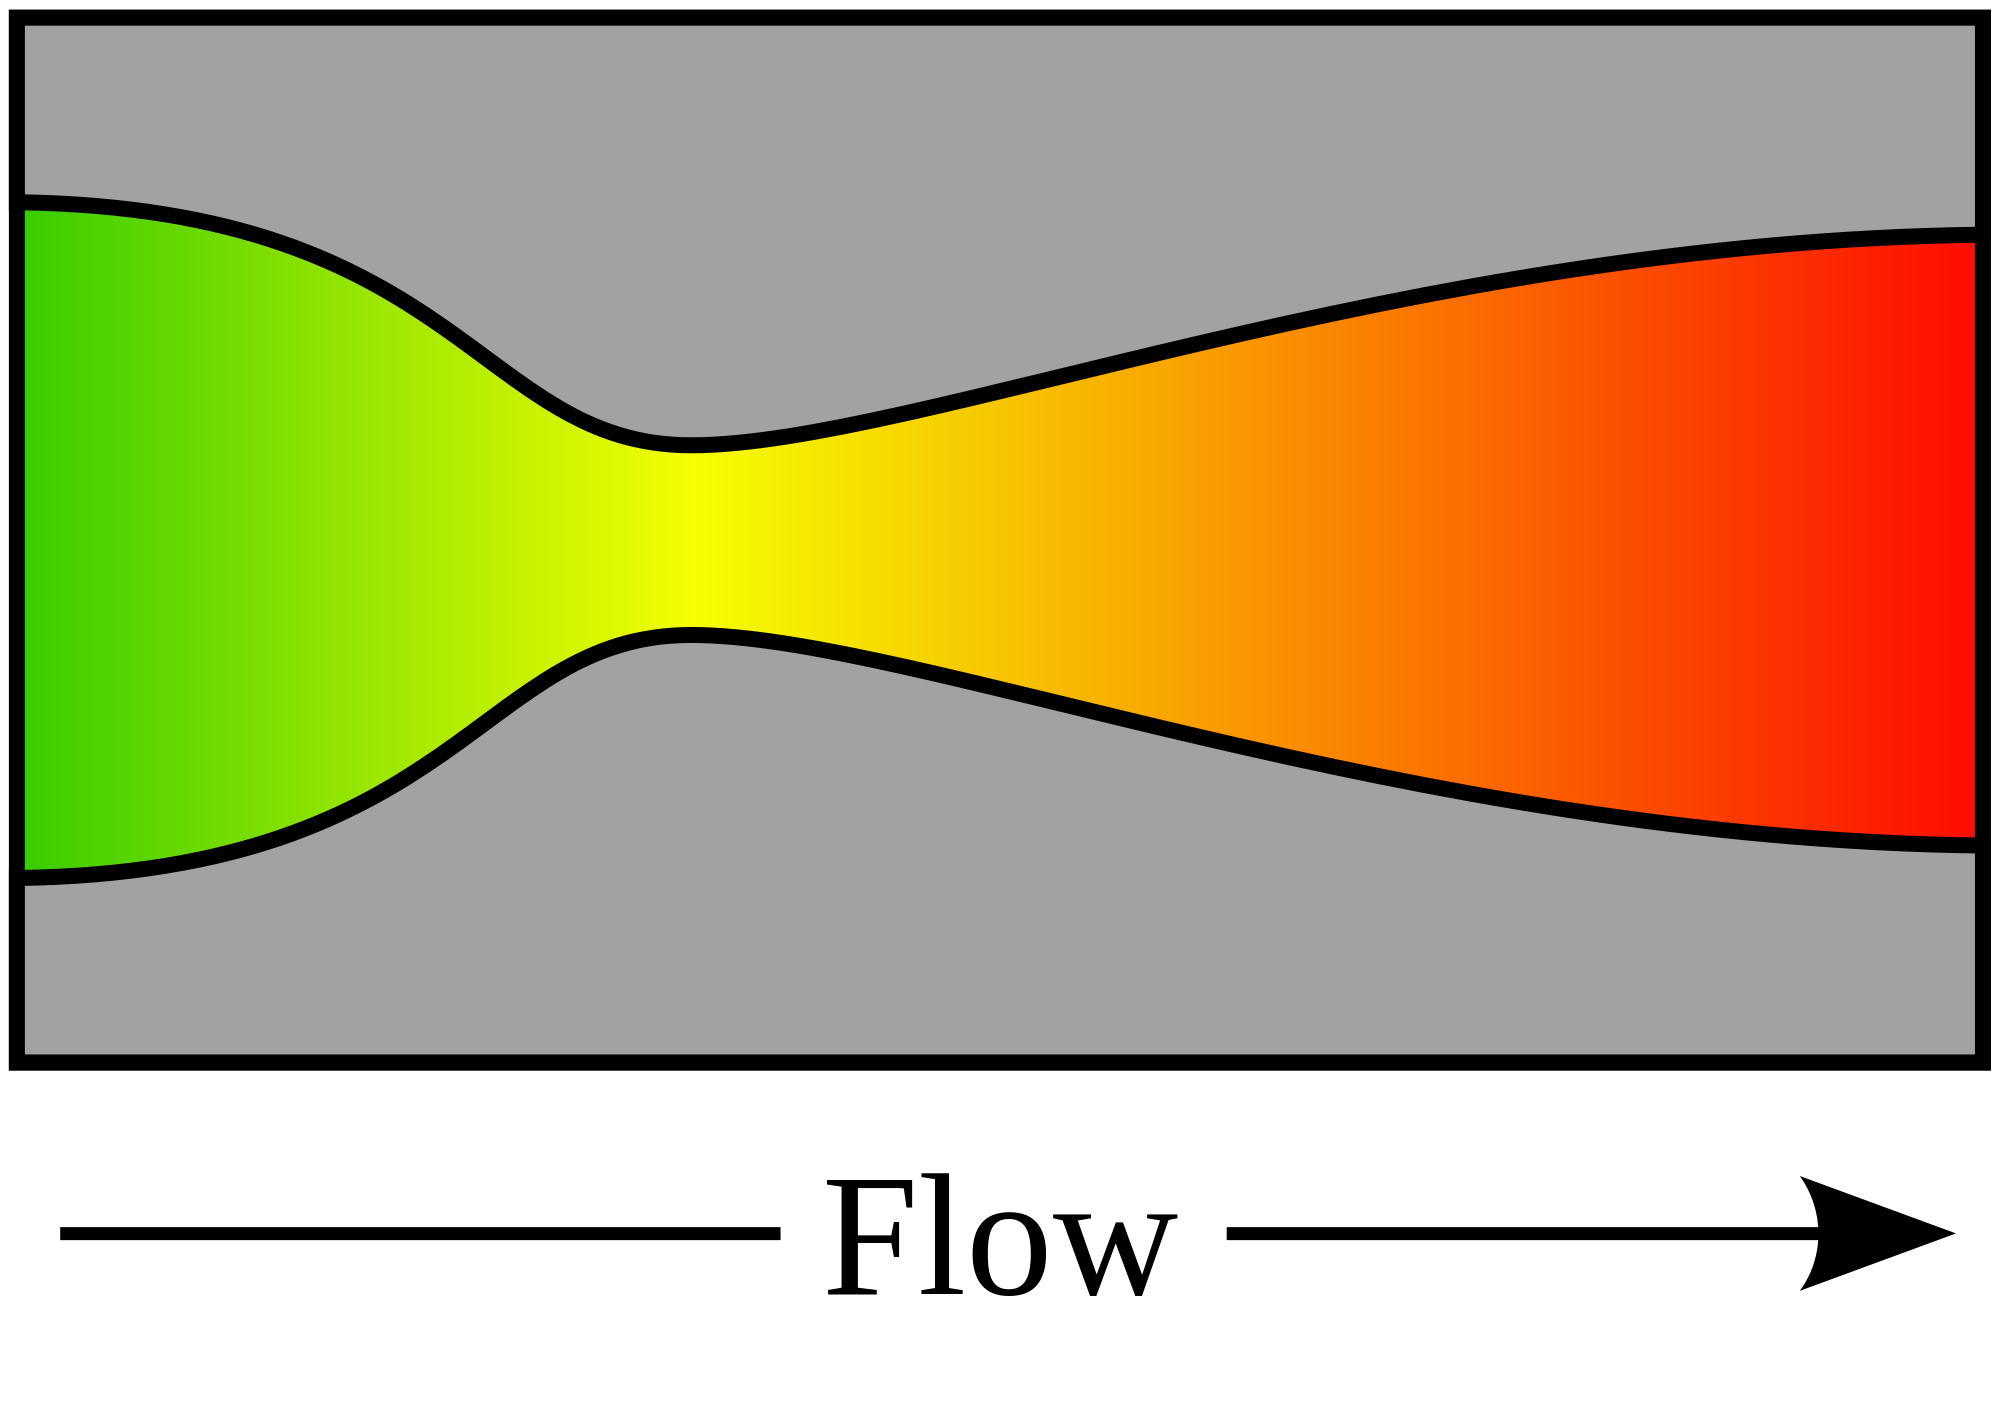
\includegraphics[width=\textwidth]{delaval}
		\caption{Schematic of a de Laval nozzle, where the green area is equivalent to the mixing chamber, and the red area is the nozzle's exit. Picture taken from \cite{wikidelaval}.}
		\label{fig:delaval}
	\end{figure}

	The rocket nozzle's primary function is to channel the combusted propellant out of the rocket and accelerate it. The optimal nozzle maximizes the velocity of the exhaust, preferably to supersonic values. The most well-known nozzle is a convergent-divergent nozzle called a de Laval Nozzle, which performs all of these things through simple geometry. Such a nozzle can be seen on figure \ref{fig:delaval}, where the combustion chamber is to the left, and the exhaust is to the right. The flow's velocity increases from green to red in the direction of the flow. An important part of maximizing the nozzle's performance is ensuring that the flow stays isentropic. Isentropic flow requires that the flow is frictionless and adiabatic, which ensures entropy is conserved. Isentropic flow is considered to \emph{only} be dependent on the cross-sectional area of the nozzle that the fluid moves through \cite{nakkanozz}. This allows calculation of any variable in any place, given some initial conditions.

	As the fluid is pushed through the throat it is highly pressurized. The nozzle is in contact with the surroundings, which acts as a reservoir of low-pressure gas between atmospheric pressure ($\SI{101.3}{kPa}$)
	and no pressure (in space!), depending on the rocket's whereabouts. The expansion of course depends on the surrounding pressure, but in general, the plume can be over-- and under--expanded and ambient. Ambient is the preferred expansion of the plume, where the exhaust gas is in pressure equilibrium with the surrounding air. If the exhaust has the same pressure as the surroundings, the gas is optimally expanded, and provides the maximum amount of thrust to the rocket \cite{robertnozzle}.

\section{Heat Capacity}

	The rocket's internal energy can be approximated as a closed system, which changes by adding heat through combustion or decomposition. Heat capacity is a measurable physical quantity, which is proportional to the ratio of heat added to the system, to the resulting change in temperature. The heat capacity ratio is denoted by $\gamma$ (or $\kappa$ by mechanical engineers), and it is given by the equation:
	 \begin{align}
		 \gamma &= \frac{C_p}{C_v}
	 \end{align}
	$\gamma$ being the ratio between $C_p$, which is the heat capacity at constant pressure, and $C_v$ which is the heat capacity at constant volume. $\gamma$ is also known as the isentropic expansion factor, which is essential in the next section \cite{IntroFluidRobert}.

	The heat capacity ratio for various gases changes with temperature, albeit very little \cite{FluidFrank}. In order to simplify the calculations, the heat capacity ratio for the rocket's fluids is assumed to be constant at $\gamma = 1.2$. This is a rather crude simplification, as the heat capacity ratio can change with upwards $\pm 0.1$ in the temperature and pressure ranges we are working. Complications with the simulation software EES did not allow a continuous recalculation in every iteration, however.

\section{Isentropic Flow}

	In order to effectively describe the rocket's behavior, we have to assume a few things:
	\begin{enumerate}[topsep=0pt,itemsep=-1ex,partopsep=1ex,parsep=1ex]
		\item{Entropy is conserved.}
		\item{Decomposition and combustion products obey the perfect gas law.}
		\item{All chemical reactions are adiabatic: No heat is lost to the surroundings.}
		\item{The fluid velocity inside the chamber is approximately zero, allowing us to assume stagnated pressure. The velocity is \emph{not} assumed to be zero when entering the throat and nozzle, however.}
	\end{enumerate}

	The assumption of isentropic flow stems from the idea that the process is reversible. The fluid will, after moving through the nozzle, have the same original values. The second law of thermodynamics states that reversible flow maintains entropy, and this allows us to calculate almost any value related to the rocket's flow. It is therefore an essential piece to the project \cite{nakkanozz}.

	If supersonic flow is not achieved by gradual means, isentropic flow is not a valid assumption. If shock waves occur abruptly, isentropic flow is not a valid assumption. Hence, exit values are simulated before any normal or oblique shock relations occur \cite{nasaisentrop}.

	The simulation is based on four valuable equations: The conservation of energy, the continuity equation, the momentum equation and equation of state.

	\begin{figure}
		
\includegraphics[width=\textwidth]{elon2}
		\caption{Isentropic flow between two points $x_1$ and $x_2$ in the rocket.}
		\label{fig:isentropicflow}
	\end{figure}


	Conservation of energy requires that for adiabatic flow, between two any points $x_1$ and $x_2$, as seen in figure \ref{fig:isentropicflow}:
	\begin{align}
		h_1 - h_2 & = \frac{1}{2} \left(v_2^2 - v_1^2 \right) = C_p (T_1 - T_2)
		\intertext{where $h$ again is the enthalpy of the fluid, $v$ is the flow velocity and $C_p$ is the heat capacity, T is the fluid's temperature. From the continuity equation, we can find a pseudo-steady state from looking at the stagnation temperature in the chamber. Setting $v_2 = 0$ yields the stagnation temperature:}
		T_0 &= T + \frac{v^2}{2 C_p}
		\intertext{This yields several key relationships between stagnation properties for pressure, density and temperature according to \cite{turbomac}:}
		\frac{T_0}{T} & = \left(\frac{P_0}{P}\right)^{\frac{\gamma-1}{\gamma}} = \left(\frac{\rho_0}{\rho}\right)^{\gamma-1}
		\intertext{Using this, we can find the temperature at the exit:}
		T_e &= T_0 \left(\frac{P_e}{P_0}\right)^{1-\frac{1}{\gamma}}
		\intertext{As $P_e$ is the exit pressure, which is equivalent to the ambient pressure. The exit temperature allows us to calculate the density of the exiting fluid $\rho_e$:}
		P_e &= \rho_e R T_e \Rightarrow \rho_e = \frac{P_e}{R T_e}
		\intertext{Bernoulli's equation provides us with the exit velocity $v_e$:}
		v_e &= \sqrt{2 \frac{P_0-P_e}{\rho_e}} = \sqrt{2 \frac{P_0-P_e}{\frac{P_e}{R T_e}}}\\
		&=  \sqrt{2 \frac{(P_0-P_e)R T_e}{P_e}}
		\intertext{Exit velocity and density yields the mass outflow per second:}
		\dot{m}_\text{out} &= A_e \cdot v_e \cdot \rho_e
	\end{align}
	and knowing how much matter is flowing "into" the rocket (see injection and combustion chamber sections) yields the total enthalpy contained in the rocket at all times. Therefore, we can now approximate the temperature in the rocket's chamber, knowing the different material's abundances. Finding the temperature of the materials
